\documentclass[mathNotesPreamble]{subfiles}
\begin{document}
%\relscale{1.4} %TODO
\section{16.1: Double Integrals over Rectangular Regions}

  \begin{center}
    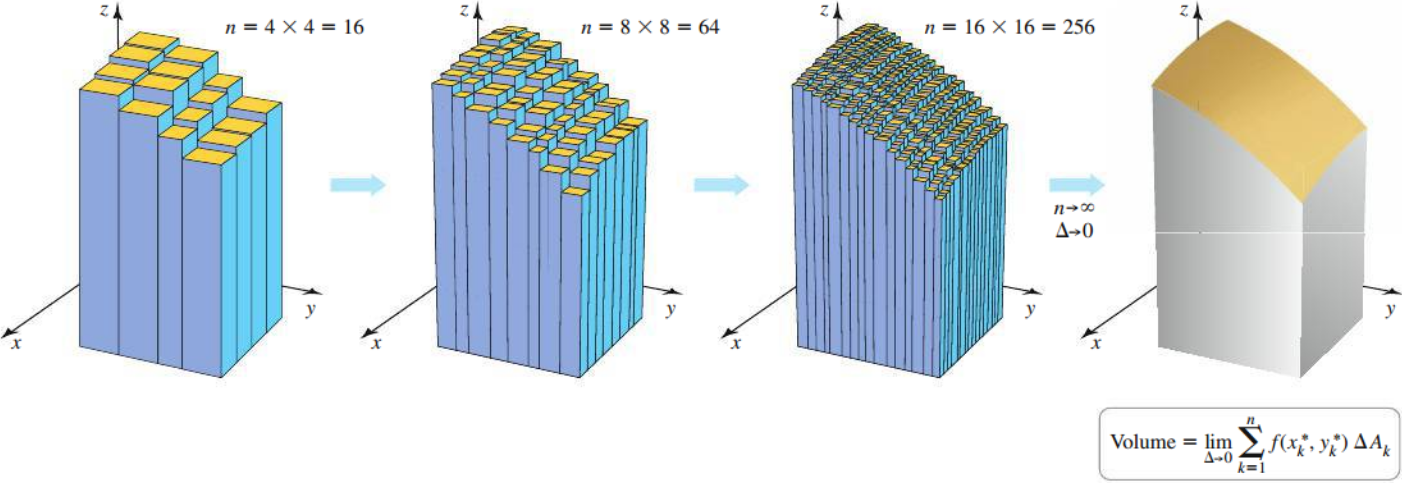
\includegraphics[width=0.975\linewidth]{images/briggs_16_01/fig16_04}
  \end{center}

  \begin{defn*}[Double Integrals]
    A function $f$ defined on a rectangular region $R$ in the $xy$-plane is \textbf{integrable} on $R$ if $\ds\lim_{\Delta\to 0} \sum\kto^n f(x_k^*, y_k^*)\, \Delta A_k$ exists for all partitions of $R$ and for all choices of $(x_k^*, y_k^*)$ within those partitions. The limit is the \textbf{double integral of $f$ over $R$}, which we write
      \[\iint\limits_R f(x,y)\,dA=\lim_{\Delta\to 0} \sum\kto^n f(x_k^*, y_k^*)\,\Delta A_k.\]
  \end{defn*}

  \begin{ex*}
    Compute the following integral: $\ds \int_0^1 \int_0^2 \parens{6-2x-y}\,dy\,dx$
  \end{ex*}
  \vspace*{\stretch{1}}
  \pagebreak

  \begin{ex*}
    Compute the following integral: $\ds \int_0^2 \int_0^1 \parens{6-2x-y}\,dx\,dy$
  \end{ex*}
  \vspace*{\stretch{1}}
  \begin{thmBox*}[Theorem 16.1: (Fubini) Double Integrals over Rectangular Regions]
    Let $f$ be continuous on the rectangular region $R=\set{(x,y):a\leq x\leq b,\ c\leq y\leq d}$. The double integral of $f$ over $R$ may be evaluated by either of the two iterated integrals:
      \[\iint\limits_R f(x,y)\,dA=\int_c^d\int_a^b f(x,y)\,dx\,dy=\int_a^b\int_c^d f(x,y)\,dy\,dx.\]
  \end{thmBox*}
  \pagebreak

  \begin{ex*}
    Find the volume of the solid bounded by the surface $f(x,y)=4+9x^2y^2$ over the region $R=\set{(x,y): -1\leq x\leq 1,\ 0\leq y\leq 2}$. Integrate with respect to $x$ first, then with respect to $y$ first.
  \end{ex*}
  \vspace{\stretch{1}}
  \pagebreak

  \begin{ex*}
    Evaluate $\ds\iint\limits_R ye^{xy}\,dA$, where $R=\set{(x,y): 0\leq x\leq 1, 0\leq y\leq \ln(2)}$.
  \end{ex*}
  \vspace*{\stretch{1}}
  \pagebreak

  \begin{defn*}[Average Value of a Function over a Plane Region]
    The \textbf{average value} of an integrable function $f$ over a region $R$ is
      \[\bar{f}=\frac{1}{\textnormal{area of }R}\iint\limits_R f(x,y)\,dA.\]
  \end{defn*}

  \begin{ex*}
    Find the average value of $f(x,y)=2-x-y$ over the region \newline $R=\set{(x,y): 0\leq x\leq 2,\ 0\leq y\leq 2}$.
  \end{ex*}
  \vspace*{\stretch{1}}

  \pagebreak
\end{document}